\documentclass[a4paper,10pt]{jsarticle}

% 数式
\usepackage{amsmath,amsfonts}
\usepackage{bm}
% 画像
\usepackage[dvipdfmx]{graphicx}
\usepackage{here}

\usepackage{listingsutf8,jlisting} %日本語のコメントアウトをする場合jlistingが必要
%ここからソースコードの表示に関する設定
\lstset{
  basicstyle={\ttfamily},
  identifierstyle={\small},
  commentstyle={\smallitshape},
  keywordstyle={\small\bfseries},
  ndkeywordstyle={\small},
  stringstyle={\small\ttfamily},
  frame={tb},
  breaklines=true,
  columns=[l]{fullflexible},
  numbers=left,
  xrightmargin=0zw,
  xleftmargin=3zw,
  numberstyle={\scriptsize},
  stepnumber=1,
  numbersep=1zw,
  lineskip=-0.5ex
}

\begin{document}

\title{ソフトウェア設計法レポート(採点希望)}
\author{坪井正太郎(101830245)}
\date{\today}
\maketitle
\section{構成要素}
ここでは、主な処理をするプログラムが、精算機を動作させるコンピュータ上で同時に動いていても、別の場所であってもいいように、内部で処理と入出力を担当する部分を「メインプログラム」として設定した。
\begin{itemize}
  \item 利用者
  \item 自動車
  \item ストッパー
  \item 精算機
  \item メインプログラム
  \item 打刻DB
\end{itemize}

\section{構成要素間の関係、システム境界}

\begin{enumerate}
  \item 利用者は、自動車でストッパーを踏んで入庫する
  \item ストッパーは、メインプログラムに入庫を通知する
  \item メインプログラムは、打刻DBに、入庫情報を登録する
  \item メインプログラムは、ストッパーに板を上げるように入力する\\
  \item 利用者は、精算機に入庫場所の識別子を入力する
  \item 精算機は、メインプログラムに識別子を入力する
  \item メインプログラムは、打刻DBから識別子に対応する入庫情報を問い合わせる
  \item 打刻DBは、メインプログラムに対応する情報を返す
  \item メインプログラムは、精算機に計算結果の料金を伝える
  \item 利用者の決済
  \item 精算機は、メインプログラムに決済が完了したら通知する
  \item メインプログラムは、打刻DBに出庫情報を登録する
  \item メインプログラムは、ストッパーに板を下げるように入力する
  \item 利用者は、自動車でストッパーを踏んで出庫する
\end{enumerate}

1~4は入庫時、5~は出庫時の動作。

システム境界は以下の図のようになる。
\begin{figure}[H]
  \centering
  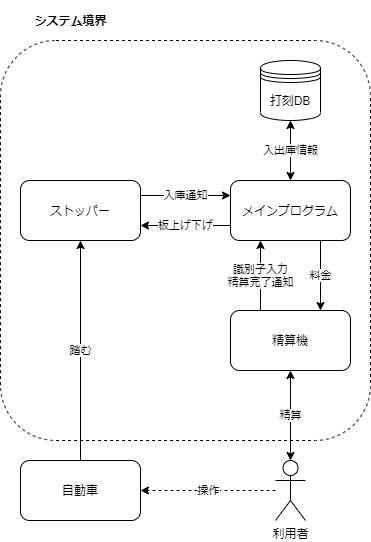
\includegraphics[width=7cm]{01.png}
\end{figure}

\section{その他の定義}
\subsection{プラットフォーム}
ストッパーには、車では反応するが人の重さには反応しないという要求がある。
精算機には、少なくとも精算機能の他に、金額を表示する機能と識別子を入力する機能を持つ必要かある。
メインプログラムを動作させるコンピュータは、時刻データを扱うので、現在時刻を取得できる必要がある。

\subsection{データ定義}
入庫情報は以下のような項目を持つ。
\begin{itemize}
  \item 入庫時刻
  \item 入庫場所の識別子
\end{itemize}

出庫情報は以下のような項目を持つ。
\begin{itemize}
  \item 出庫時刻
  \item 出庫場所の識別子
  \item 徴収料金
\end{itemize}

\subsection{アルゴリズム}
想定されるアルゴリズムは以下(料金計算は考えられる一例を示した)
\begin{itemize}
  \item 日時の差分取得
  \item 日時の差分から料金を計算
  \begin{itemize}
    \item 日時を設定した単位時間で割る
    \item あまりは切り捨てて、結果と単位料金をかける
  \end{itemize}
\end{itemize}

\end{document}
